%%%%%%%%%%%%%%%%
%% Preambule  %%
%%%%%%%%%%%%%%%%

\documentclass[11pt]{article}

\usepackage{amsmath,amsfonts,amssymb}
\usepackage{upgreek}
\usepackage{enumerate}
\usepackage{enumitem}   %
\usepackage{multicol}
\usepackage{scrextend}
\usepackage{fancyhdr}
\usepackage{lastpage}
\usepackage{subcaption} % 2 column images
\usepackage[all]{xy}
\usepackage{tikz-qtree}
\usepackage[margin=2.5cm]{geometry}
\input{../../Template/fitch.sty}

\setlength{\parindent}{0pt}

\pagestyle{fancy}

\lhead{\opdrachtNaam\ \opdrachtNummer}
\rhead{\naam(\studentNummer)}
\rfoot{Pagina\ \thepage\ van\ \pageref{LastPage}}
\lfoot{\datum}
\cfoot{}

\renewcommand\headrulewidth{0.4pt}
\renewcommand\footrulewidth{0.4pt}

\newcommand{\E}{\exists}
\newcommand{\A}{\forall}

\newcommand{\ccen}[2]{\llap{$#1$}${}\mathrel{\circ}{}$\rlap{$#2$}}

%%%%%%%%%%%%%%
%% Gegevens %%
%%%%%%%%%%%%%%

\newcommand{\naam}          {Stefan Schenk}
\newcommand{\studentNummer} {11881798}
\newcommand{\opdrachtNaam}  {Assignment}
\newcommand{\opdrachtNummer}{3}
\newcommand{\datum}         {November 2017}

%%%%%%%%%%%%%%%%
%% Antwoorden %%
%%%%%%%%%%%%%%%%

\begin{document}

% Opgaven:
%
% The exercises for Homework 3 are:
%  5.31(g), 5.32(2,3), 5.33(2), 5.37(2,3, van rechts naar links), 5.38(3), 5.53(Quine dolk)

\subsection*{Opgave 5.31}

%  Hint for exercise 5.31(g): For the last step of the proof, you need to use the rule G V (gebruik rule for the disjunction) with phi_1 = q and phi_2 = r and psi is the formula (p ∧ q) ∨ (p ∧ r).

(g) $p\wedge(q\vee r) \vdash (p\wedge q)\vee(p\wedge r)$

\[
\begin{nd}
  \hypo {1} {p\wedge(q\vee r)}  \by{ass}{}
  \have {2} {p}                 \ae{1}
  \have {3} {(q\vee r)}         \ae{1}
  \open
  \hypo {4} {q}                 \by{ass}{}
  \have {5} {(p\wedge q)}       \ai{2, 4}
  \have {6} {(p\wedge q) \vee (q \vee r)} \oi{5}
  \close
  \open
  \hypo {7} {r}                 \by{ass}{}
  \have {8} {(p\wedge r)}       \ai{2, 7}
  \have {9} {(p\wedge q) \vee (q \vee r)} \oi{8}
  \close
  \have {10} {(p\wedge q) \vee (q \vee r)} \oi{1, 6, 9}
\end{nd}
\]

\subsection*{Opgave 5.32}

(2) $p\wedge (q\wedge r) \vdash r \wedge p$

\[
\begin{nd}
  \hypo {1} {p\wedge (q\wedge r)}   \by{ass}{}
  \have {2} {p}                     \ae{1}
  \have {3} {(q \wedge r)}          \ae{1}
  \have {4} {r}                     \ae{3}
  \have {5} {(r \wedge p)}          \ai{2, 4}
\end{nd}
\]

(3) $p \rightarrow (q\wedge r), q \rightarrow s, p\vdash s$

\[
\begin{nd}
  \hypo {1} {p \rightarrow (q\wedge r)}   \by{ass}{}
  \hypo {2} {q \rightarrow s}             \by{ass}{}
  \hypo {3} {p}                           \by{ass}{}
  \have {4} {(q \wedge r)}                \ie{1, 3}
  \have {5} {q}                           \ae{4}
  \have {6} {s}                           \ie{2, 5}
\end{nd}
\]

\pagebreak

\subsection*{Opgave 5.33}

(2) $\varphi\vee(\psi\wedge\chi);
  (\varphi\vee\psi)\wedge(\varphi\vee\chi)$

\begin{center}
  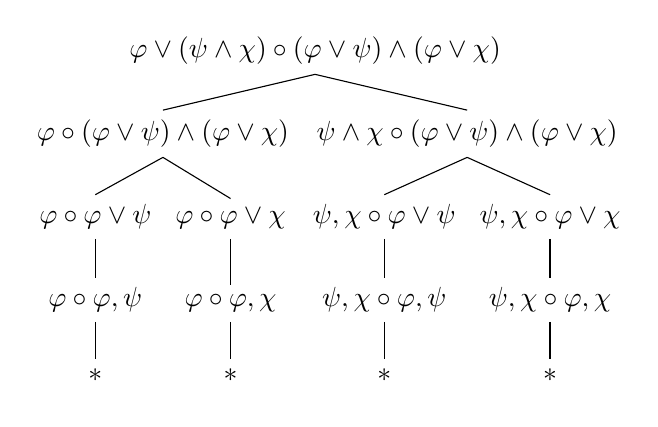
\begin{tikzpicture}
    \Tree [.
      $\varphi\vee(\psi\wedge\chi)\circ(\varphi\vee\psi)\wedge(\varphi\vee\chi)$
        [.$\varphi\circ(\varphi\vee\psi)\wedge(\varphi\vee\chi)$
          [.$\varphi\circ\varphi\vee\psi$ [.$\varphi\circ\varphi,\psi$ [.* ]]]
          [.$\varphi\circ\varphi\vee\chi$ [.$\varphi\circ\varphi,\chi$ [.* ]]]
        ]
      [.$\psi\wedge\chi\circ(\varphi\vee\psi)\wedge(\varphi\vee\chi)$
        [.$\psi,\chi\circ\varphi\vee\psi$ [.$\psi,\chi\circ\varphi,\psi$ [.* ]]]
        [.$\psi,\chi\circ\varphi\vee\chi$ [.$\psi,\chi\circ\varphi,\chi$ [.* ]]]
      ]
    ]
  \end{tikzpicture}
\end{center}

\subsection*{Opgave 5.37}

(2) $\varphi\leftrightarrow\psi;
  (\varphi\rightarrow\psi)\wedge(\psi\rightarrow\varphi)$

\begin{center}
  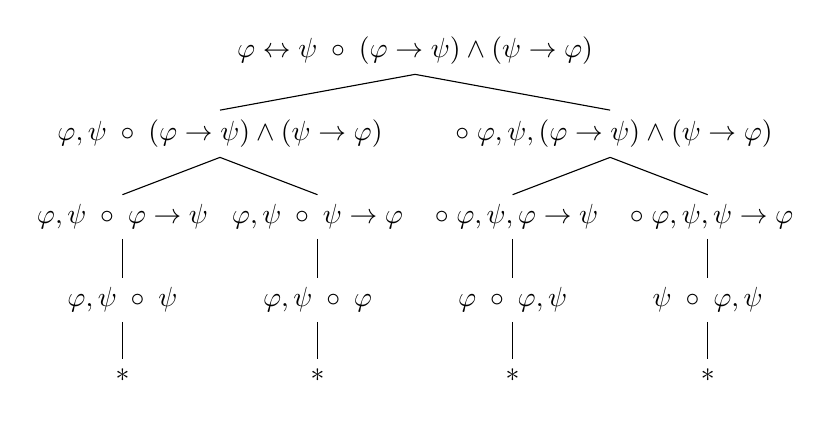
\begin{tikzpicture}
    \Tree [
      .$\varphi\leftrightarrow\psi\;\circ\;(\varphi\rightarrow\psi)\wedge
        (\psi\rightarrow\varphi)$
        [
          .$\varphi,\psi\;\circ\;(\varphi\rightarrow \psi)\wedge(\psi\rightarrow \varphi)$
          [
            .$\varphi,\psi\;\circ\;\varphi\rightarrow \psi$
            [
              .$\varphi,\psi\;\circ\;\psi$
              [
                .*
              ]
            ]
          ] [
            .$\varphi,\psi\;\circ\;\psi\rightarrow \varphi$
            [
              .$\varphi,\psi\;\circ\;\varphi$
              [
                .*
              ]
            ]
          ]
        ] [
          .$\;\circ\;\varphi,\psi,(\varphi\rightarrow \psi)\wedge
          (\psi\rightarrow \varphi)$
          [
            .$\;\circ\;\varphi,\psi,\varphi\rightarrow \psi$
            [
              .$\varphi\;\circ\;\varphi,\psi$
              [
                .*
              ]
            ]
          ] [
            .$\;\circ\;\varphi,\psi,\psi\rightarrow \varphi$
            [
              .$\psi\;\circ\;\varphi,\psi$
              [
                .*
              ]
            ]
          ]
        ]
    ]
  \end{tikzpicture}
\end{center}

(3) $\varphi\rightarrow\psi;
  \neg\psi\rightarrow\neg\varphi$

\begin{center}
  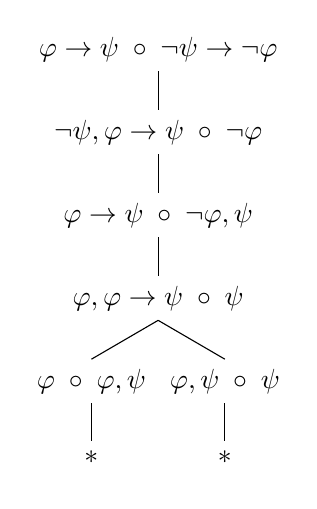
\begin{tikzpicture}
    \Tree [
      .$\varphi\rightarrow\psi\;\circ\;\neg\psi\rightarrow\neg\varphi$
        [
          .$\neg\psi,\varphi\rightarrow\psi\;\circ\;\neg\varphi$
          [
            .$\varphi\rightarrow\psi\;\circ\;\neg\varphi,\psi$
            [
              .$\varphi,\varphi\rightarrow\psi\;\circ\;\psi$
              [
                .$\varphi\;\circ\;\varphi,\psi$
                [
                  .*
                ]
              ] [
                .$\varphi,\psi\;\circ\;\psi$
                [
                  .*
                ]
              ]
            ]
          ]
        ]
    ]
  \end{tikzpicture}
\end{center}

\pagebreak

\subsection*{Opgave 5.38}

(3) $((p\rightarrow q)\wedge(q\rightarrow r))\rightarrow(p\rightarrow r)$

\begin{center}
  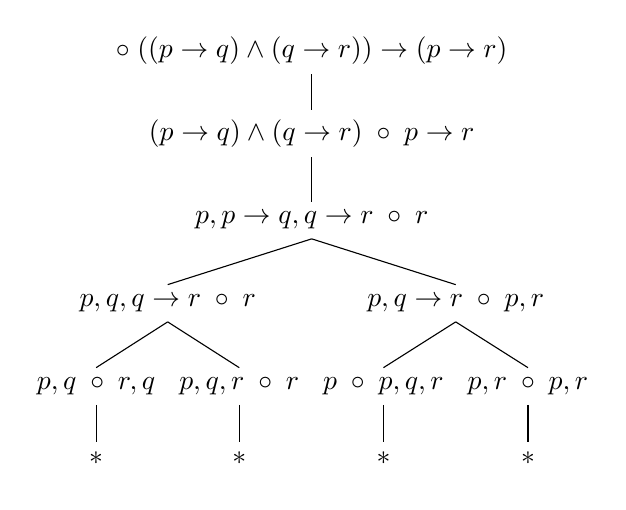
\begin{tikzpicture}
    \Tree [
      .$\circ\;((p\rightarrow q)\wedge(q\rightarrow r))\rightarrow(p\rightarrow
      r)$
      [
        .$(p\rightarrow q)\wedge(q\rightarrow r)\;\circ\;p\rightarrow r$
        [
          .$p,p\rightarrow q,q\rightarrow r\;\circ\;r$
          [
            .$p,q,q\rightarrow r\;\circ\;r$
            [
              .$p,q\;\circ\;r,q$
              [.* ]
            ] [
              .$p,q,r\;\circ\;r$
              [.* ]
            ]
          ] [
            .$p,q\rightarrow r\;\circ\;p,r$
            [
              .$p\;\circ\;p,q,r$
              [.* ]
            ] [
              .$p,r\;\circ\;p,r$
              [.* ]
            ]
          ]
        ]
      ]
    ]
  \end{tikzpicture}
\end{center}

\subsection*{Opgave 5.53}

\textit{Geef de semantische tableauregels voor de Quine dolk $\dagger$.}

\begin{itemize}

  \item $\dagger$ - links
  \begin{center}
    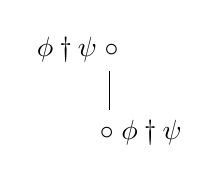
\begin{tikzpicture}
      \Tree [.$\phi\dagger\psi\;\circ\qquad\;$
        [.$\qquad\;\circ\;\phi\dagger\psi$ ] ]
    \end{tikzpicture}
  \end{center}

  \item $\dagger$ - rechts
  \begin{center}
    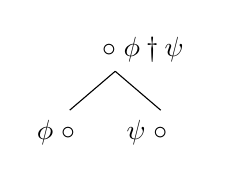
\begin{tikzpicture}
      \Tree [.$\;\qquad\circ\;\phi\dagger\psi\;$
        [.$\phi\;\circ\quad$ ] [.$\psi\;\circ\quad$ ] ]
    \end{tikzpicture}
  \end{center}

\end{itemize}

\end{document}
